\documentclass[a4paper,12pt]{article}

% Any percent sign marks a comment to the end of the line

% Every latex document starts with a documentclass declaration like this
% The option dvips allows for graphics, 12pt is the font size, and article
%   is the style

\usepackage[pdftex]{graphicx}
%\usepackage{url}
\usepackage{hyperref}
% These are additional packages for "pdflatex", graphics, and to include
% hyperlinks inside a document.
\usepackage{lettrine}
%\setlength{\oddsidemargin}{0.25in}
%\setlength{\textwidth}{6.5in}
%\setlength{\topmargin}{0in}
%\setlength{\textheight}{8.5in}

% These force using more of the margins that is the default style
\usepackage{times}
\usepackage{mathptmx}
\usepackage{color}
\usepackage{amssymb}
\usepackage{amsmath}
\usepackage{indentfirst}
\usepackage{float}
\begin{document}

% Everything after this becomes content
% Replace the text between curly brackets with your own

\title{Spring 2018 CS304 Software Engineering\\Function as a Service}
\author{Ziqiang Li\quad Yulian Mao\quad Xizi Ni\quad Yilin Zheng\quad Chenyu Zhou\\
\small \{11510352, 11510086, 11510602, 11510506, 11510374\}@mail.sustc.edu.cn\\
Stone Tencent\\
Yuqun Zhang\quad zhangyq@sustc.edu.cn}
\date{\today}

% You can leave out "date" and it will be added automatically for today
% You can change the "\today" date to any text you like


\maketitle

% This command causes the title to be created in the document

\section{Abstract}
Serverless computing is recently raised hot fields of cloud computing. Serverless computing can hide the implementation of the back end from developers or users by using API gateway. The FaaS is a widely used model of serverless computing. In this project, we focus on developing serverless cloud functions based on Tencent Cloud to provide a service for massive data. This service is also planned to integrate into WeChat App so that provides an easier and wider range of application.  

\section{Introduction}
Cloud computing is popularized since Amazon released its EC2 in 2006. The past few years have seen the rapid developments of cloud computing, the models of cloud computing have changed both in its architectures and its orientation. The most recent hot topics raised from this field is widely-known \textbf{Serverless Computing}. Such a name makes this model a little ambiguous for the general public and the latest architecture \textbf{FaaS} is also little known to the public. However, more and more people are using these servers either consciously or unconsciously. They break through the wall of local computing and support more powerful online services such as online language translation, navigation, and so on.

\subsection{From IaaS to FaaS}
The following figures simply display the developments of models of cloud computing\cite{models}. The details of the models can be referred in Appendix~\ref{sec:appendix3}

\begin{figure}[H]
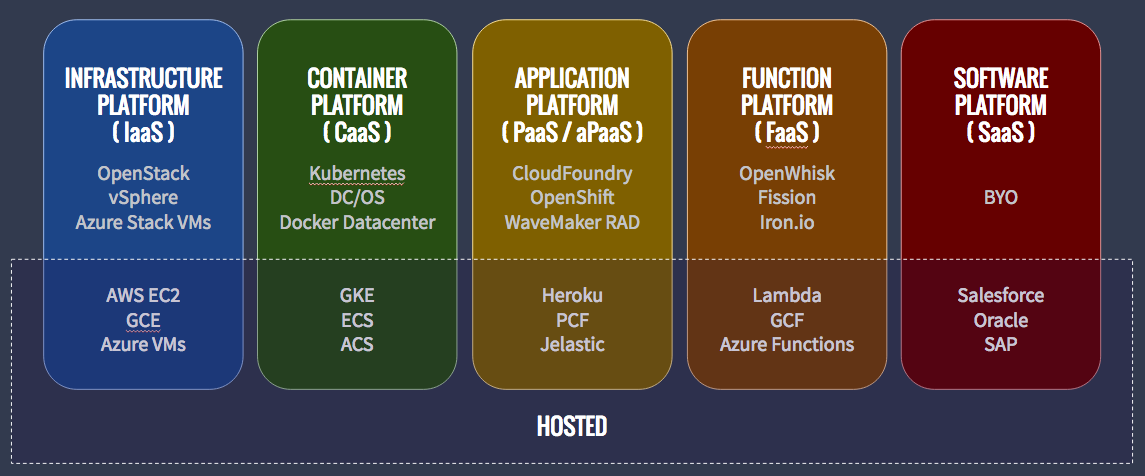
\includegraphics[scale=0.337]{figures/platform-spectrum-small.png}
\caption{Examples of Cloud Platforms}
\end{figure}

\begin{figure}[H]
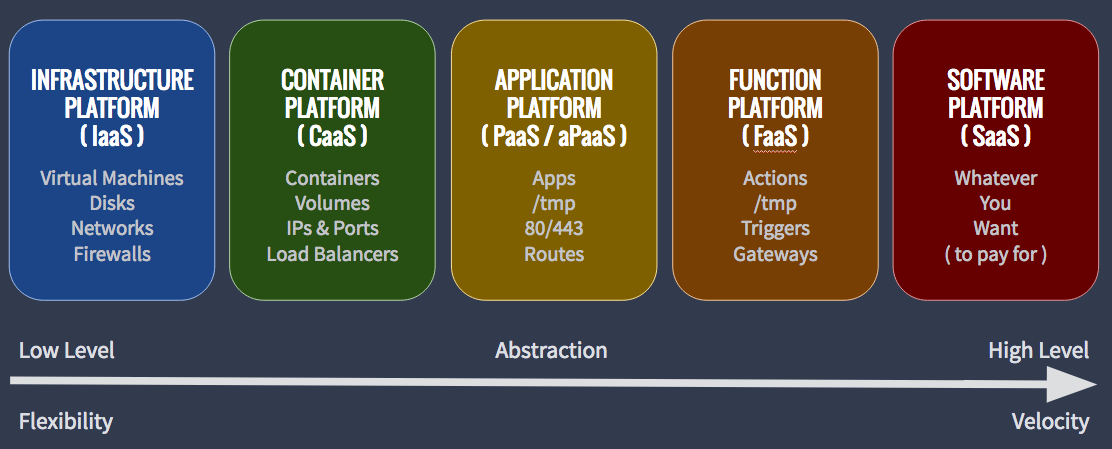
\includegraphics[scale=0.345]{figures/cloud-platform-abstration.png}
\caption{Cloud Platforms, their interfaces, and the scale of abstraction}
\end{figure}


\subsection{Serverless Computing}
Serverless computing is a cloud computing model in which the cloud provider dynamically manages the allocation of machine resources. The pricing is based on the actual amount of resources consumed by an application or requests, instead of the units of capacity. Serverless computing does not mean no servsers, it still requires servers. The name "serverless computing" is used because the server management and capacity planning decisions are completely hidden from the developers or operators. Serverless code can be used in conjunction with code deployed in traditional styles, such as microservices. Alternatively, applications can be written to be purely serverless and use no provisioned servers at all\cite{serverless}.

\subsection{Function as a Service}
Function as a service (FaaS) is a category of cloud computing services that provides a platform allowing customers to develop, run, and manage application functionalities without the complexity of building and maintaining the infrastructure typically associated with developing and launching an app. Building an application following this model is one way of achieving a "serverless" architecture, and is typically used when building microservices applications\cite{faas}. 

The advantages of FaaS:
\begin{itemize}
	\item Lower cost: save infrastructure costs, personnel cost, and development costs
	\item Strong expandability
	\item Simpler management
	\item High resource utilization
\end{itemize}

Developments of FaaS:
\begin{itemize}
	\item 2014: First made available to the world by \textsl{hook.io}
	\item 2016: \textsl{AWS Lambda}, \textsl{Google Cloud Functions}, \textsl{Microsoft Azure Functions}, \textsl{IBM/Apache's OpenWhisk}(open source)
	\item 2017: \textsl{Oracle Cloud Fn}(open source)
\end{itemize}

Nowadays more domestic companies provides FaaS including \textsl{Alibaba Cloud}, \textsl{Tencent Cloud}, and \textsl{Qiniu Cloud}.

\subsection{API Gateway}

The Figures~\ref{fig:apigateway} shows the simple structure of API Gateway.
\begin{figure}[H]
\centering
\label{fig:apigateway}
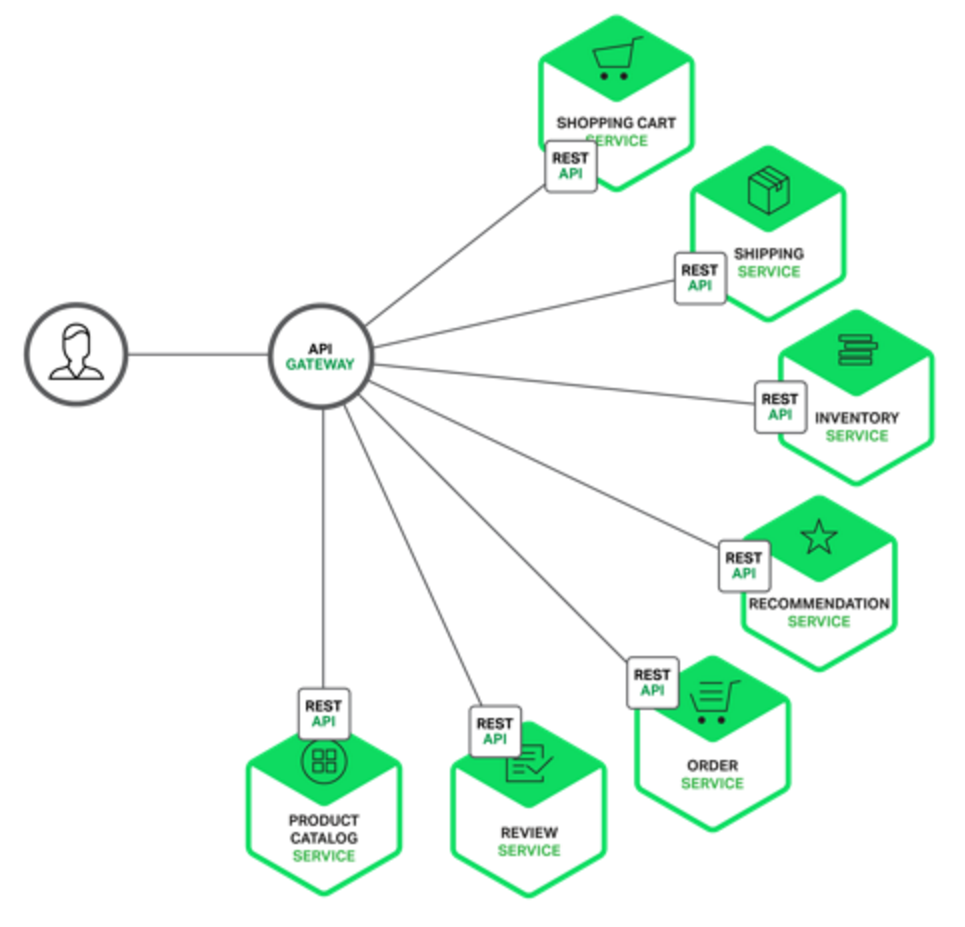
\includegraphics[scale=0.281]{figures/api-gateway.png}
\caption{API Gateway}
\end{figure}

Compare to the traditional API usage in Appendix~\ref{sec:api}, the services are hidden from users and only exposure simple and uniform APIs for users. 

\section{Requirements}
Our project based on the problem we mentioned in the previous section. In order to deal with the unstable user demand. The providers can not expend their server unlimited. Therefore, the FaaS is suitable for their scenario. Based on this background, the stakeholder required us to implement some figure modification cloud function such as:
\begin{itemize}
    \item Zoom in / out figure
    \item Lossless zoom in
    \item Figure Cutting
    \item Watermark (words or figures)
    \item Round Corner
    \item Overlap QCodes
\end{itemize}

Besides, those functions should be highly customized. The software providers can easily embed or transfer those function into their system. 

After we finish those figure modification cloud functions, we want to add some interesting cloud function into our project due to the reason that FaaS is suitable for the function which requires a lot of computation which is impractical in a mobile terminal. The interesting functions may include style migration or face correlation analysis. 

In addition to the cloud functions developing, we decided that we can embed those cloud function to WeChat APP or H5 Web page to release our product and test whether our cloud function can deal with massive data.

\section{Architecture}

The architecture can be referred as \ref{diagram}.

\begin{figure}[H]
\label{diagram}
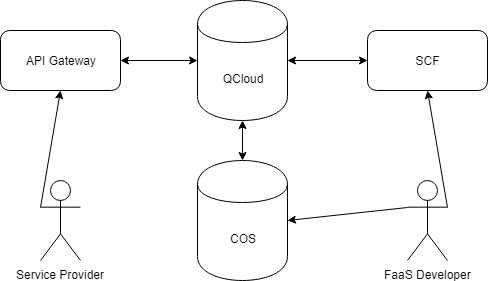
\includegraphics[scale=0.8]{figures/Diagram.png}
\caption{Architecture}
\end{figure}

Thanks for the Tencent Cloud, our project is based on their cloud servers. We use their SCF service to develop our cloud function, use their COS to store figures and use API Gateway to custom our APIs to release to users. 

\section{Implementation}

\subsection{Team assignment}

\begin{itemize}
	\item Front End: Yulian Mao, Chenyu Zhou, Xizi Ni
	\item Back End: Ziqiang Li, Yulian Mao, Yilin Zheng
	\item WeChat App: Yulian Mao, Chenyu Zhou, Yilin Zheng, Xizi Ni, Ziqiang Li
\end{itemize}

\subsection{Timeline}
Before Opening Report
\begin{itemize}
	\item Communicate with stakeholder and finish requirement analysis
	\item Study QCloud service
	\item Finish Architecture Design
\end{itemize}
Before Middle Report
\begin{itemize}
	\item Finish Figure Processing Cloud Function Development
	\item Design APIs
	\item Finish Front End Development
\end{itemize}
Before Final Report
\begin{itemize}
	\item Testing our SCF with massive data
	\item Release APIs to users in QCloud
\end{itemize}

\begin{figure}[H]
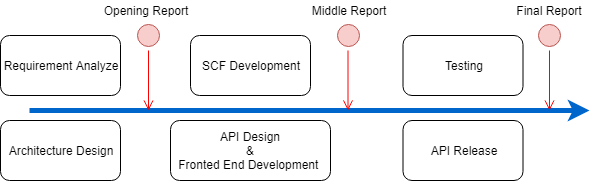
\includegraphics[scale=0.6]{figures/Timeline.png}
\caption{Timeline}
\end{figure}

\subsection{Platform choices}
	The platform we choices includes Tencent Cloud Servers, API Gateway, and COS Object storage. The system is Linux.

\section{Conclusion}
This project is a serverless function development based on Tencent Cloud with extended functionality such as the combination of this services and WeChat App. This service provides basic image processing, style transform and can be further added more SCFs if necessary. This service is serverless so the users have not burden of managing and maintaining servers. Besides, the pricing is counted by the times of requests but not whole servers which largely saves their cost. The combination of this service and WeChat App provides more channels for users to meet their demand.

\appendix

\section{Cloud Computing Models}
\label{sec:appendix3}
The following four figures comes from \cite{models}
\begin{figure}[H]
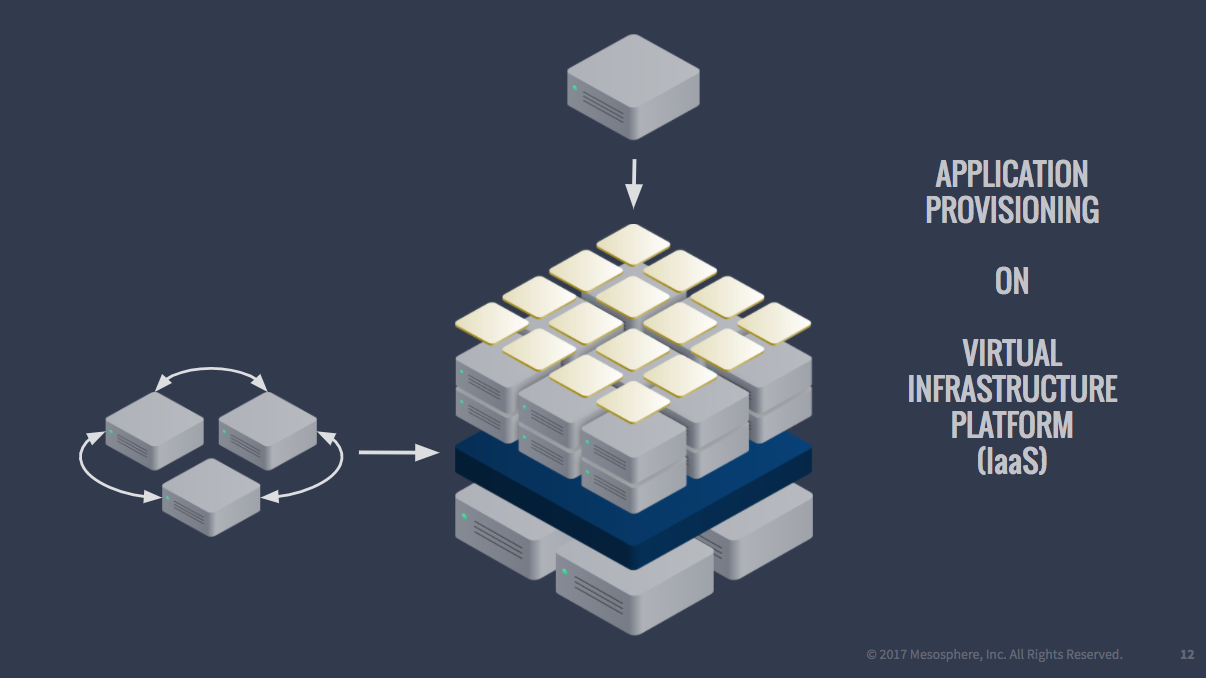
\includegraphics[scale=0.32]{figures/IaaS.png}
\caption{IaaS}
\end{figure}
\begin{figure}[H]
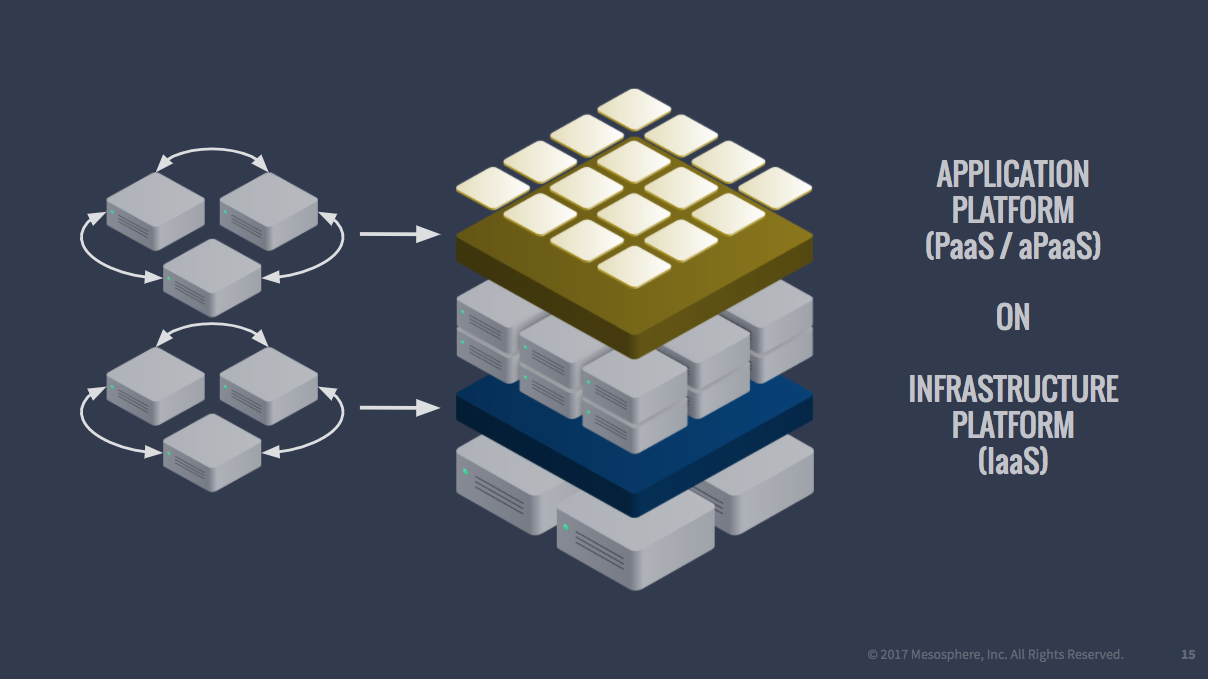
\includegraphics[scale=0.32]{figures/PaaS-IaaS.png}
\caption{PaaS-IaaS}
\end{figure}
\begin{figure}[H]
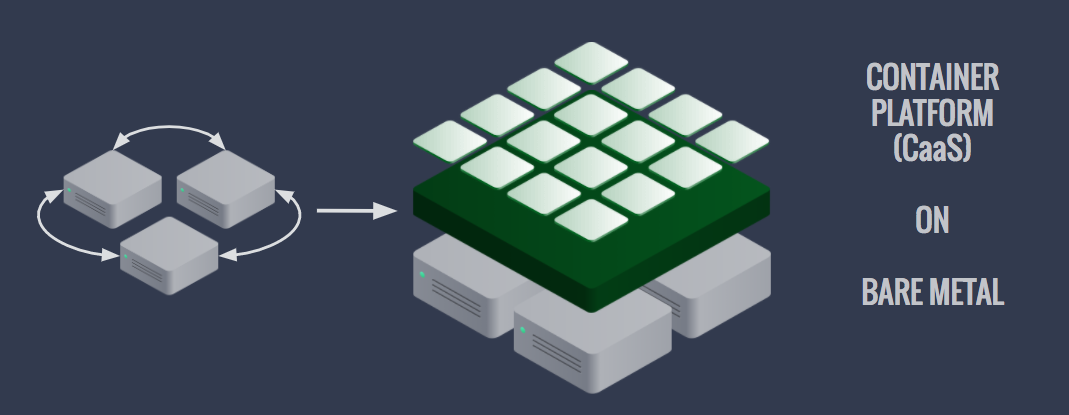
\includegraphics[scale=0.361]{figures/CaaS-Metal.png}
\caption{CaaS-Metal}
\end{figure}
\begin{figure}[H]
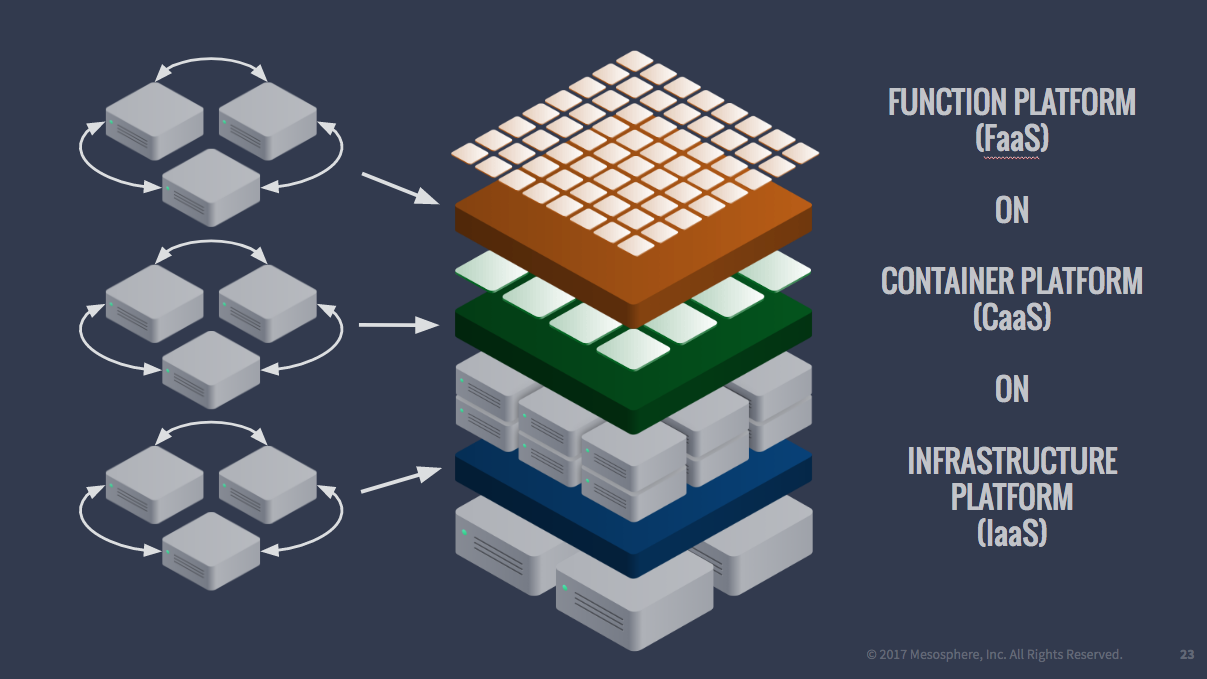
\includegraphics[scale=0.32]{figures/FaaS-CaaS-IaaS.png}
\caption{FaaS-CaaS-IaaS}
\end{figure}

\section{APIs Usage}
\label{sec:api}
\begin{figure}[H]
\label{fig:api}
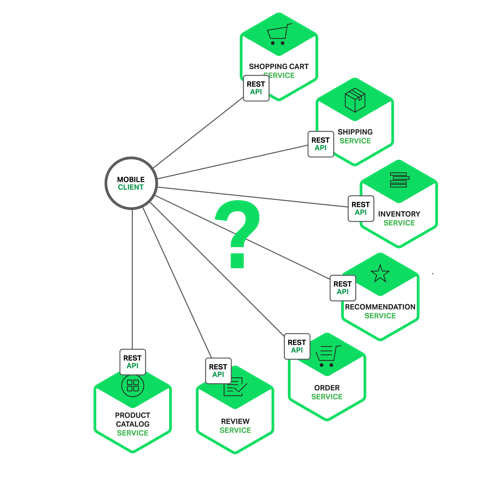
\includegraphics[scale=0.7]{figures/api.png}
\caption{Traditional APIs usages}
\end{figure}

\begin{thebibliography}{1}
\bibitem{serverless}
https://en.wikipedia.org/wiki/Serverless\_computing
\bibitem{faas}
https://en.wikipedia.org/wiki/Function\_as\_a\_service
\bibitem{models}
https://mesosphere.com/blog/iaas-vs-caas-vs-paas-vs-faas/

\end{thebibliography}
\end{document}
